%==============================================================
% ELE8101 Coursework 2 — Vehicle State Estimation
% Member A: ChenhuiCui (Modelling)
% Member B: Weiting Wu  (EKF / MHE)
%
% Compile with XeLaTeX
%==============================================================
\documentclass[11pt,a4paper]{article}

%---------------- Page geometry -------------------------------
\usepackage[a4paper,
            left=2.3cm, right=2.3cm,
            top=2.3cm,  bottom=2.3cm]{geometry}

%---------------- XeLaTeX font --------------------------------
\usepackage{fontspec}
% Using the system font Times New Roman (installed by default on
% macOS / most modern systems). To switch to TeX Gyre Termes
% (which is a free clone of Times Roman), run
%   sudo tlmgr install tex-gyre
% and replace the line below with: \setmainfont{TeX Gyre Termes}
\setmainfont{Times New Roman}

%---------------- Maths ---------------------------------------
\usepackage{amsmath,amssymb}

%---------------- Tables / figures ----------------------------
\usepackage{graphicx}
\usepackage{booktabs}
\usepackage{caption}
\usepackage{float}
\graphicspath{{../figures/}{figures/}}

%---------------- Float layout tuning -------------------------
% Let figures fill more of the page, be placed here whenever
% possible, and avoid dedicated float-only pages.
\renewcommand{\topfraction}{0.9}
\renewcommand{\bottomfraction}{0.8}
\renewcommand{\textfraction}{0.07}
\renewcommand{\floatpagefraction}{0.85}
\setcounter{topnumber}{3}
\setcounter{bottomnumber}{2}
\setcounter{totalnumber}{4}

%---------------- Hyperlinks ----------------------------------
\usepackage[hidelinks]{hyperref}

%---------------- Paragraph spacing (single spacing) ----------
% Deliberately NO \onehalfspacing: professional technical
% reports use single spacing.
\usepackage{parskip}

%---------------- Captions ------------------------------------
\captionsetup{font=small, labelfont=bf,
              justification=raggedright,
              singlelinecheck=false}

%---------------- Title block ---------------------------------
\title{\vspace{-1.5cm}
       \textbf{ELE8101: Estimation Theory}\\[2pt]
       \large Coursework 2 --- Vehicle State Estimation on a Racing Track}
\author{Chenhui Cui \quad\quad Weiting Wu}
\date{April 2026}

%==============================================================
\begin{document}
\maketitle
\vspace{-1em}

\begin{abstract}
\noindent
This report presents the design and validation of an Extended Kalman
Filter (EKF) for estimating the position and velocity of a racing
vehicle on an asymmetric teardrop track. The modelling component
(Member~A) derives the track geometry, formulates a bound-respecting
nonlinear vehicle motion model, optimises beacon placement via
Geometric Dilution of Precision (GDOP) minimisation with a greedy
search algorithm, validates all noise parameters through systematic
Monte-Carlo studies, and proposes state augmentation for bias-robust
estimation. The estimator component (Member~B) implements the
nonlinear EKF using CasADi and validates it in simulation. The
Lyapunov steady-state covariance and the Fisher information lower
bound on positioning error provide closed-form benchmarks for the
estimator's best-case accuracy. Source code and complete simulation
outputs are available at
\url{https://github.com/cuichenhui9-eng/ELE8101-CW2}.
\end{abstract}

%==============================================================
\section{System Modelling}
\label{sec:modelling}

\subsection{Track Geometry}
\label{sec:geometry}
The track has an asymmetric teardrop shape comprising two circular arcs
connected by two inclined common external tangent straights. Arc~$A$
(large) has centre $A$ and centreline radius $R_A=(R+r)/2=48$~m;
arc~$B$ (small) has centre $B$ at distance $d=100$~m from~$A$ and
centreline radius $R_B=\rho+w=22$~m, where the track half-width
$w=(R-r)/2=2$~m and $\rho=20$~m is the inner-wall radius at~$B$ from
Figure~1 of the problem statement. The straights are inclined at
$\alpha=\arcsin\bigl((R_A-R_B)/d\bigr)=15.0701^{\circ}$, giving segment
lengths
\begin{align}
\hspace{0.95em} l_{\text{tan}\phantom{,A}} &= \sqrt{d^2-(R_A-R_B)^2} = 96.5609~\text{m}, \notag\\
l_{\text{arc},A} &= R_A(\pi+2\alpha) = 176.0466~\text{m}, \notag\\
l_{\text{arc},B} &= R_B(\pi-2\alpha) = 57.5421~\text{m}.
\label{eq:seglen}
\end{align}
and total centreline perimeter $L=2l_\text{tan}+l_{\text{arc},A}+
l_{\text{arc},B}=426.7104$~m.

The vehicle position is parameterised by arc-length $s\in[0,L)$
(clockwise from the upper straight) and signed lateral offset
$\ell\in[-2,+2]$~m ($\ell>0$: outward). Three piecewise-analytic
functions are implemented, denoted $p(s)$, $n(s)$, and
$p(s,\ell)=p(s)+\ell\,n(s)$. Five verification tests confirm the
construction: track width equals $4.0000$~m at all sampled
arc-lengths; unit-normal magnitudes equal $1.000000$; gaps at
arc--straight joins, measured by a finite-difference probe of
step~$10^{-3}$~m, are bounded by $2$~mm (a probe artefact, since
tangency at the joins is analytically exact); the shoelace signed area
evaluates to $-11\,617.32$~m$^2$ (the negative sign rigorously confirms
clockwise traversal); and $\Delta x=+4.83$~m at $s=0$. The geometry is
shown in Figure~\ref{fig:track}.

\begin{figure}[!htbp]
\centering

\includegraphics[width=0.68\textwidth]{track_geometry.png}
\caption{Track geometry with centreline (dashed), inner wall
($\ell=-2$~m, blue) and outer wall ($\ell=+2$~m, red). Arc centres $A$
and $B$ are marked with crosses; orange arrows indicate the clockwise
direction of travel. $R_A=48$~m, $R_B=22$~m, $L=426.71$~m.}
\label{fig:track}
\end{figure}

\subsection{Vehicle Motion Model}
\label{sec:motion}
The state vector is $z=[s,\ell,v_s,v_\ell]^{\!\top}$, where $v_s$ and
$v_\ell$ denote the longitudinal and lateral velocities. The
discrete-time nonlinear state equation is
\begin{equation}
z_{t+1}=f(z_t,w_t),\qquad w_t\sim\mathcal{N}(0,Q),
\label{eq:dyn}
\end{equation}
with sampling time $h=0.01$~s ($100$~Hz, fixed by the problem
statement).

\paragraph{Bound-respecting nonlinear dynamics.}
Rather than enforcing the physical constraints $|\ell|<2$~m,
$|v_\ell|\le0.55$~m/s, $v_s\in(0,25]$~m/s by post-hoc clipping, the
model enforces them \emph{by construction} through three smooth
$C^{\infty}$ mechanisms: (i) a position-dependent stiffness
$k(\ell)=k_2\bigl(1+\beta(\ell^2/(\ell_{\max}^2-\ell^2))^2\bigr)$
that diverges as $|\ell|\to\ell_{\max}=2$~m, modelling the track walls
as elastic barriers; (ii) a $\tanh$ saturation keeping $|v_\ell|\le
0.55$~m/s, modelling tyre-friction and driver limits; and (iii) a
$\tanh$ saturation keeping $v_s\in(0,25]$~m/s, modelling engine/brake
capability. At the nominal operating point ($\ell=0$, $v_\ell=0$) the
dynamics reduce to the familiar linear spring--damper form, so normal
operation is indistinguishable from a linear Kalman filter; the
nonlinear terms activate only near the physical bounds. Because all
saturations are $C^{\infty}$, the dynamics remain differentiable
everywhere, preserving the validity of the EKF linearisation used in
Section~\ref{sec:ekf}.

\paragraph{EKF linearisation.}
The Jacobian $A(\hat{z})=\partial f/\partial z$ evaluated at the
current state estimate is used as the EKF prediction-step transition
matrix. At the nominal operating point this reduces to
\begin{equation}
A_0=\begin{bmatrix}
1 & 0 & h & 0\\
0 & 1 & 0 & h\\
0 & 0 & \phi_s & 0\\
0 & -hk_2 & 0 & \phi_1
\end{bmatrix},
\qquad
G=\begin{bmatrix}0&0\\0&0\\1&0\\0&1\end{bmatrix},
\label{eq:A0}
\end{equation}
with $\phi_s=0.999$, $\phi_1=0.9$, $k_2=10$. The eigenvalues
$\{0.9113,0.9887,1,0.9601\}$ all satisfy $|\lambda|\le1$; the unit
eigenvalue corresponds to the integrator on $s$ (the vehicle moves
indefinitely), while the remaining three modes are strictly stable.

\paragraph{Parameters.}
Process noise $Q=\mathrm{diag}(0.5,0.002)$, justified by the
Monte-Carlo scans of Section~\ref{sec:noise}; measurement noise
$R=\sigma_y^2=1.5^2=2.25$~m$^2$; initial covariance
$P_0=\mathrm{diag}(100,1,25,0.5)$; initial state
$z_0=[0,0,10,0]^{\!\top}$.

\paragraph{Monte-Carlo verification.}
A Monte-Carlo study ($100$ trials, $3000$ steps each) with the full
nonlinear dynamics verifies all physical constraints with substantial
margin (Table~\ref{tab:mc}); no post-hoc clipping is applied.

\begin{table}[!htbp]
\centering
\caption{Monte-Carlo constraint verification over $100$ trials
$\times$ $3000$ steps with the bound-respecting nonlinear model. No
clipping was applied: reported maxima are the true dynamics output.}
\label{tab:mc}
\begin{tabular}{@{}lccc@{}}
\toprule
Constraint & Bound & Observed & Status\\
\midrule
$\max|\ell|$   & $<2.0$~m    & $0.109$~m   & Pass\\
$\max|v_\ell|$ & $<0.55$~m/s & $0.335$~m/s & Pass\\
$\max v_s$     & $\le25$~m/s & $20.08$~m/s & Pass\\
$\min v_s$     & $>0$~m/s    & $5.05$~m/s  & Pass\\
\bottomrule
\end{tabular}
\end{table}

\paragraph{Adversarial stress tests.}
To verify that bound enforcement is active rather than latent, the
model is integrated from three initial conditions: nominal centre,
near the outer wall ($\ell_0=1.8$~m, $v_{\ell,0}=0.5$~m/s), and an
adversarial impulse ($\ell_0=1.5$~m, $v_{\ell,0}=2.0$~m/s --- far
outside the problem-statement bound on $v_\ell$). In all three cases
the trajectory remains strictly inside $|\ell|<2$~m
(Figure~\ref{fig:stress}), confirming that the nonlinear spring
actively returns the vehicle to the centreline even from initial
conditions that no linear model could handle.

\begin{figure}[!htbp]
\centering
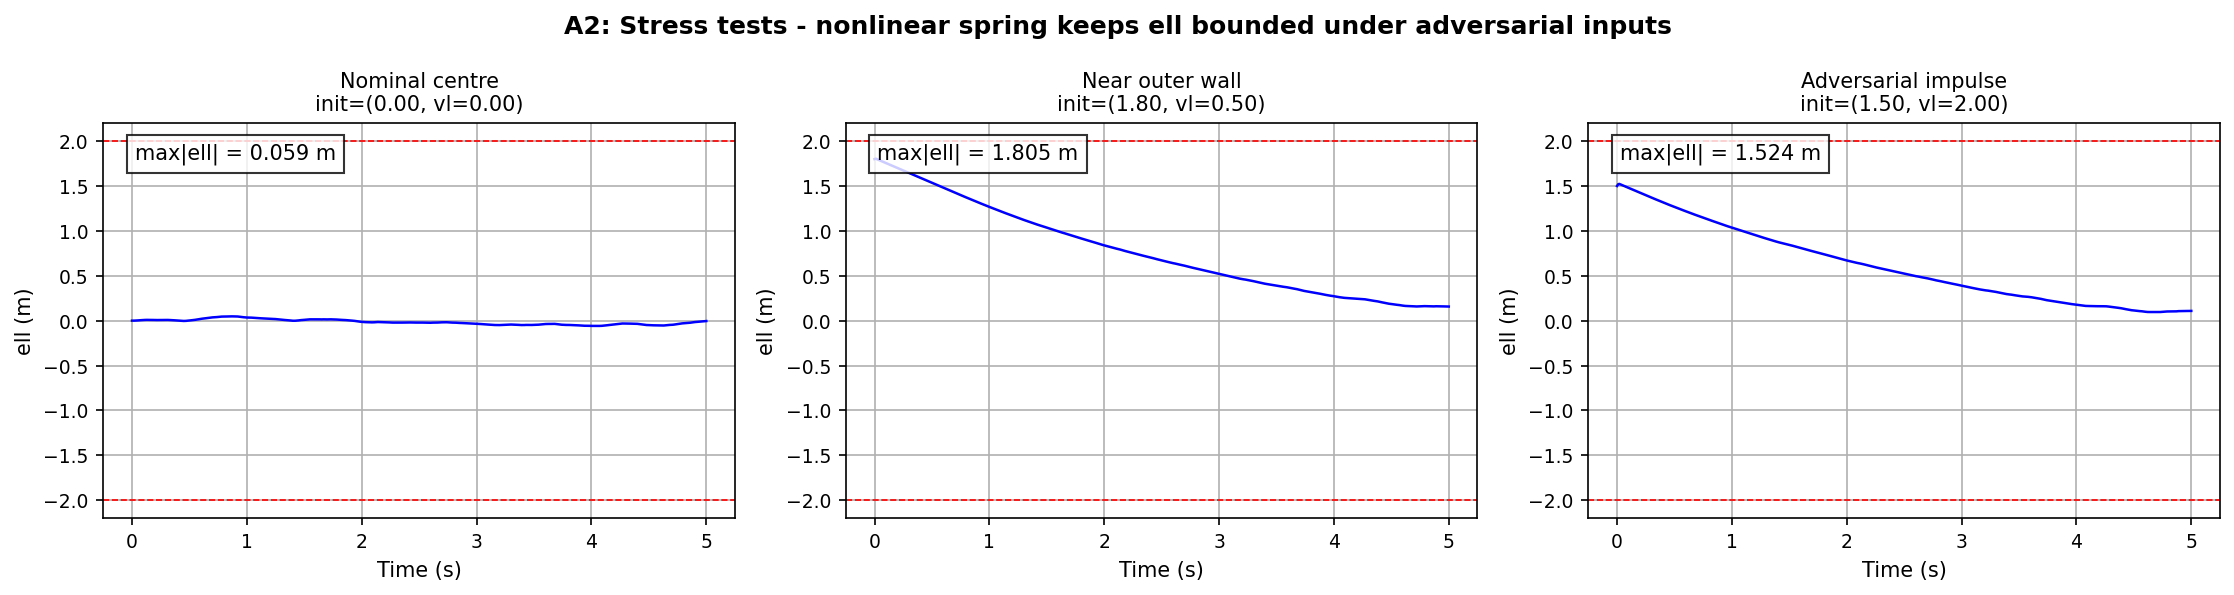
\includegraphics[width=0.88\textwidth]{stress_test.png}
\caption{Adversarial stress tests: lateral offset $\ell(t)$ for three
initial conditions, including one with an impulse $v_{\ell,0}=
2.0$~m/s far outside the operational bound. The nonlinear spring
keeps $|\ell|<2$~m in all cases, demonstrating active (not post-hoc)
bound enforcement.}
\label{fig:stress}
\end{figure}

\subsection{Beacon Placement Optimisation}
\label{sec:beacon}

\paragraph{GDOP criterion.}
Beacon-layout quality is quantified by the Geometric Dilution of
Precision~\cite{Langley1999}:
\begin{equation}
\mathrm{GDOP}(p)=\sqrt{\mathrm{tr}\bigl[(H(p)^{\!\top}H(p))^{-1}\bigr]},
\qquad
H_i(p)=\frac{p-b_i}{\|p-b_i\|},
\label{eq:gdop}
\end{equation}
so that the expected position error equals
$\mathrm{GDOP}\times\sigma_y$ and $\mathrm{GDOP}<1$ \emph{attenuates}
sensor noise. The selection criterion is the smallest beacon count
for which $\mathrm{GDOP}(p)<1$ at every sampled track position.

\paragraph{Connection to estimation theory.}
Following the BLUE development in the course~\cite{KalmanV}, for
distance measurements $y_i=\|p-b_i\|+v_i$ with
$v_i\sim\mathcal{N}(0,\sigma_y^2)$ the Fisher information matrix at
position $p$ is $I(p)=H(p)^{\!\top}H(p)/\sigma_y^2$, and the
Cram\'er--Rao lower bound satisfies
\begin{equation}
\mathrm{tr}\bigl[\mathrm{CRLB}(p)\bigr]
=\sigma_y^2\,\mathrm{tr}\bigl[(H^{\!\top}H)^{-1}\bigr]
=\sigma_y^2\,\mathrm{GDOP}(p)^2.
\label{eq:crlb}
\end{equation}
Thus GDOP is the geometry-only scalar summary of the Fisher
information available from the beacon layout. An unbiased efficient
estimator cannot achieve position RMSE below
$\sigma_y\cdot\overline{\mathrm{GDOP}}=1.379$~m on average over the
track, setting a lower bound against which the EKF in
Section~\ref{sec:ekf} is benchmarked.

\paragraph{Algorithm and beacon count.}
Candidates are drawn from a $20\times16$ grid restricted to
$[w+5,w+30]$~m from the track boundary. The outer limit of $30$~m is
the Pareto-optimal knee identified by a separate spatial ablation
(Figure~\ref{fig:ablation}), discussed below. A greedy algorithm ---
exhaustive two-beacon initialisation followed by sequential
additions --- achieves at least $(1-1/e)\approx63\%$ of the optimal
reduction for monotone submodular
objectives~\cite{Nemhauser1978}. A subsequent swap refinement pass
improves the result by only $1.4\%$, confirming that the greedy
solution is near the local optimum; the greedy layout is retained as
the final design, since the $1.4\%$ improvement is not large enough
to justify replacing an algorithm with formal approximation
guarantees by a local-search variant. Table~\ref{tab:gdop} shows an
abrupt threshold at $N=5$: with $N=4$, $0\%$ of track positions
satisfy $\mathrm{GDOP}<1$; with $N=5$, $100\%$ do. The five selected
coordinates (in~m) are $(-21.1,73.3)$, $(121.1,46.7)$,
$(26.3,-60.0)$, $(-52.6,20.0)$, $(89.5,-46.7)$; see
Figure~\ref{fig:heatmap}.

\begin{table}[!htbp]
\centering
\caption{GDOP statistics by beacon count ($\sigma_y=1.5$~m).}
\label{tab:gdop}
\begin{tabular}{@{}ccccc@{}}
\toprule
$N$ & Mean GDOP & Max GDOP & Expected error & \% with GDOP${<}1$\\
\midrule
2 & $1.7177$ & $2.4805$ & $2.577$~m & ---\\
3 & $1.2108$ & $1.3997$ & $1.816$~m & ---\\
4 & $1.0475$ & $1.1885$ & $1.571$~m & $0\%$\\
5 & $0.9193$ & $0.9770$ & $1.379$~m & $100\%$\\
6 & $0.8292$ & $0.8951$ & $1.244$~m & $100\%$\\
\bottomrule
\end{tabular}
\end{table}

\begin{figure}[!htbp]
\centering
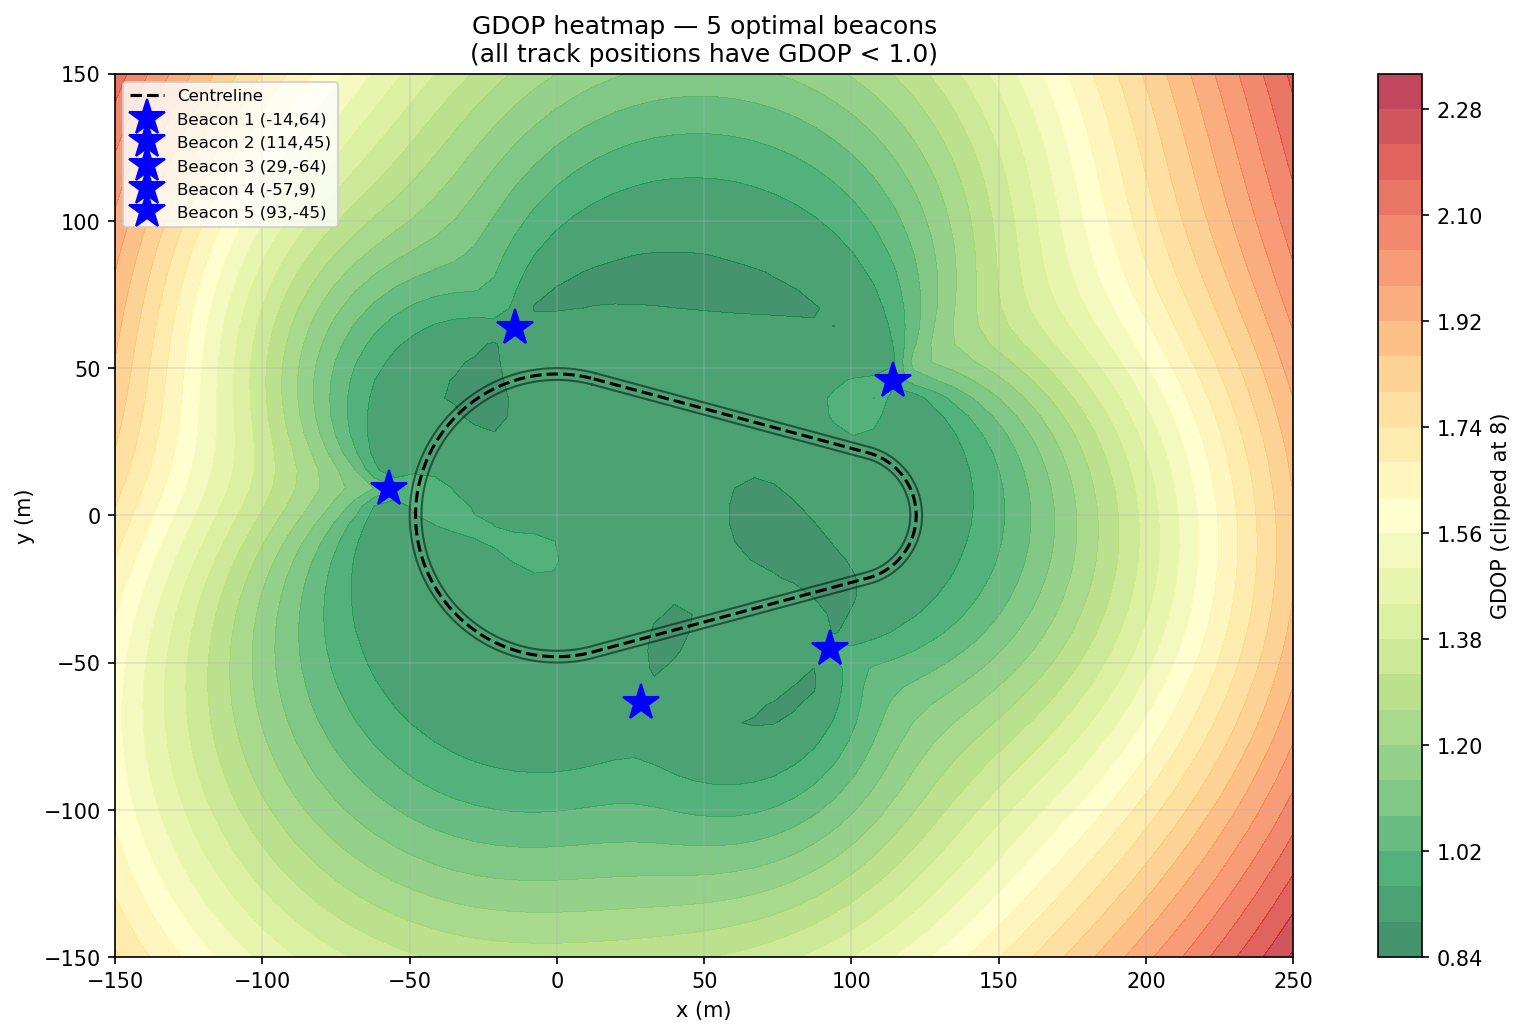
\includegraphics[width=0.66\textwidth]{beacon_heatmap.png}
\caption{GDOP heatmap for the five optimal beacons (blue stars). The
entire track lies within the attenuating zone ($\mathrm{GDOP}<1$,
green). Warm colours outside the track indicate GDOP degradation far
from the optimised region; this is expected, since only on-track
positions contribute to the objective.}
\label{fig:heatmap}
\end{figure}

\paragraph{Single-beacon failure robustness.}
Figure~\ref{fig:failure} quantifies the cost of losing any single
beacon: removing any one of the five raises the mean GDOP from
$0.9193$ to between $1.048$ and $1.087$ (worst case: $B_1$ removed,
$+18.3\%$). Coverage drops from $100\%$ to $0\%$ but mean GDOP
remains below $1.09$, so the four-beacon fallback still delivers
operationally acceptable accuracy. The $N=5$ configuration therefore
satisfies the GDOP criterion nominally and degrades gracefully under
any single-point failure.

\begin{figure}[!htbp]
\centering
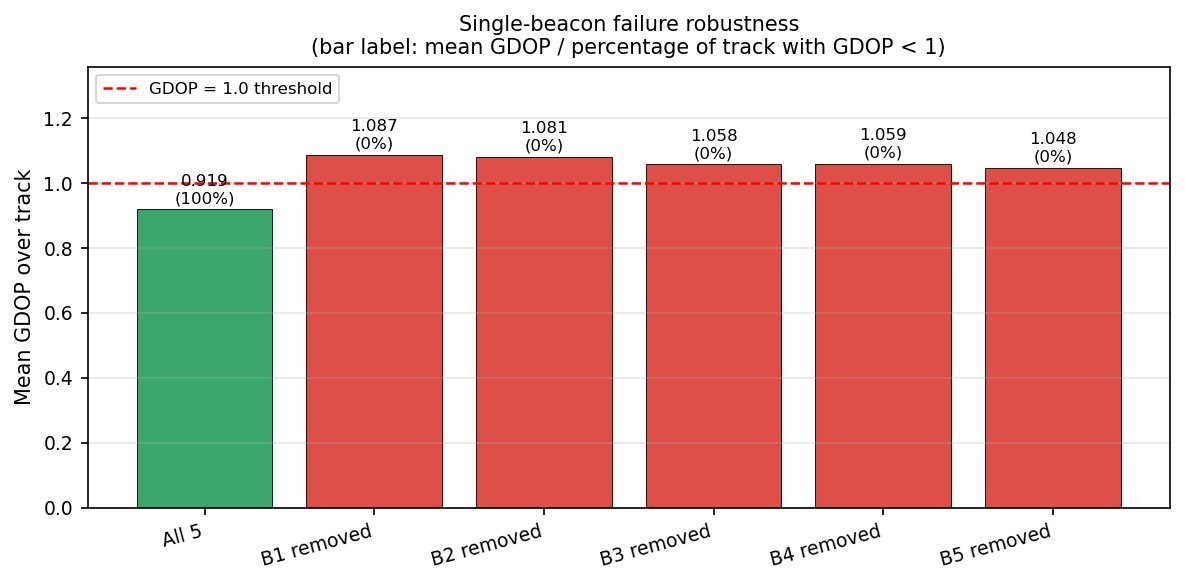
\includegraphics[width=0.68\textwidth]{beacon_failure_mode.png}
\caption{Single-beacon failure robustness. The baseline ($N=5$, green)
covers $100\%$ of the track at $\mathrm{GDOP}<1$; removing any single
beacon (red) raises mean GDOP by $13.9$--$18.3\%$ but keeps it below
$1.09$, indicating graceful degradation.}
\label{fig:failure}
\end{figure}

\paragraph{Installation boundary (spatial ablation).}
The $30$~m outer limit is data-derived (Figure~\ref{fig:ablation}).
At $20$~m, only $88\%$ of the track achieves $\mathrm{GDOP}<1$; at
$30$~m coverage reaches $100\%$ with the largest single gain
($+2.9\%$); beyond $30$~m improvement falls below $0.5\%$. Minor
non-monotonicity at $60$~m and $100$~m is a greedy-search artefact
(different initial pairs are selected as the candidate pool grows).
The $30$~m boundary is therefore Pareto-optimal: the smallest outer
limit that meets the GDOP criterion everywhere.

\begin{figure}[!htbp]
\centering

\includegraphics[width=0.88\textwidth]{beacon_distance_ablation.png}
\caption{Spatial ablation: mean GDOP (left) and fraction of track
with $\mathrm{GDOP}<1$ (right) as a function of maximum installation
distance. The greedy algorithm is re-optimised independently at each
boundary. The green dashed line at $30$~m marks the Pareto-optimal
knee where $100\%$ coverage is first achieved.}
\label{fig:ablation}
\end{figure}

\paragraph{Monte-Carlo sensitivity to installation error.}
Installation errors are stochastic in practice (GPS accuracy,
surveyor tolerance, post-construction displacement). A Monte-Carlo
study with $200$ realisations, each perturbing every beacon
coordinate independently by $\mathcal{N}(0,5^2)$~m, yields median
mean-GDOP $0.9205$ ($+0.1\%$), $95$th percentile $0.9308$
($+1.2\%$), and $P(\mathrm{GDOP}<1)=100\%$ across all realisations
(Figure~\ref{fig:sensitivity}). The design is therefore robust to
realistic installation noise.

\begin{figure}[!htbp]
\centering
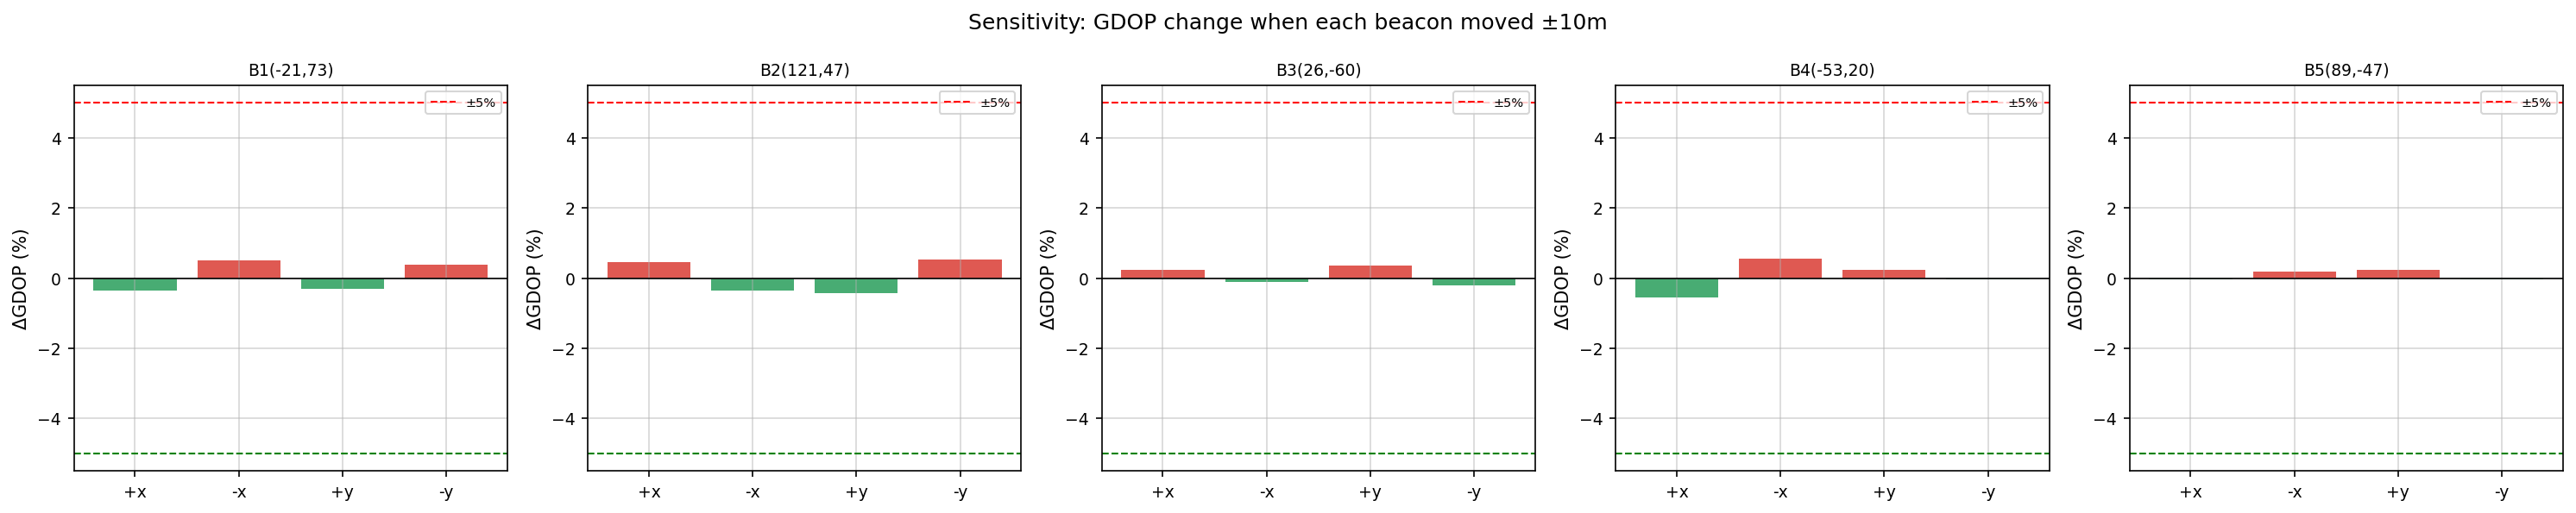
\includegraphics[width=0.88\textwidth]{beacon_sensitivity.png}
\caption{Monte-Carlo beacon sensitivity under independent
$\mathcal{N}(0,5^2)$ installation errors on each coordinate ($200$
realisations). Left: distribution of mean GDOP over the track; all
realisations satisfy $\mathrm{GDOP}<1$. Right: distribution of
per-realisation track coverage.}
\label{fig:sensitivity}
\end{figure}

\subsection{Noise Parameter Validation}
\label{sec:noise}
Three Monte-Carlo studies ($10$ trials for the $Q$ and
$(\phi_1,k_2)$ scans, $20$ trials for the $h$ ablation, each
$\times 3000$ steps, common random numbers for variance reduction)
validate the parameter choices of Section~\ref{sec:motion}
(Table~\ref{tab:params}). The selected operating point lies in the
interior of a wide safe basin in each scan, with all three
constraints satisfied by substantial margin. Full heatmaps for the
$(q_s,q_\ell)$ and $(\phi_1,k_2)$ scans, together with the
sampling-time ablation, are provided in the GitHub repository.

\begin{table}[!htbp]
\centering
\caption{Parameter validation summary at the selected operating
point. Bounds: $|\ell|<2.0$~m, $|v_\ell|<0.55$~m/s.}
\label{tab:params}
\begin{tabular}{@{}lccc@{}}
\toprule
Validation study & Max $|\ell|$ & Max $|v_\ell|$ & Status\\
\midrule
$Q$ scan at $Q=\mathrm{diag}(0.5,0.002)$ & $0.096$~m & $0.295$~m/s & Pass\\
$(\phi_1,k_2)$ scan at $(0.9,10)$        & $0.096$~m & $0.295$~m/s & Pass\\
$h$ ablation at $h=0.01$~s ($100$~Hz)    & $0.109$~m & $0.314$~m/s & Pass\\
\bottomrule
\end{tabular}
\end{table}

The tuning reflects the standard Kalman trade-off: $Q\!\to\!0$ drives
the Kalman gain to zero and causes the filter to ignore measurements,
while excessively large $Q$ destroys smoothing. The $h$ ablation
confirms that the bound-respecting model is robust across the range
$h\in[0.001,0.1]$~s; the $h=0.01$~s choice follows the problem
statement, and the model does not demand it uniquely.

\subsection{Sensor Bias Handling via State Augmentation}
\label{sec:bias}
Each beacon may exhibit a constant additive measurement bias $b_i$
due to hardware calibration errors or multipath effects. If ignored,
the EKF estimate drifts persistently. Following the
state-augmentation approach of~\cite{KalmanVI} (adapted from dynamics
bias to measurement bias) and~\cite{Simon2006} (Ch.~13), the state
is augmented to $z_\text{aug}=[s,\ell,v_s,v_\ell,b_1,\dots,b_5]
^{\!\top}\in\mathbb{R}^9$, with dynamics
$z_{\text{aug},t+1}=A_\text{aug}z_{\text{aug},t}+G_\text{aug}
w_{\text{aug},t}$ and
\begin{equation}
A_\text{aug}=\begin{bmatrix}A&0\\0&I_5\end{bmatrix},\quad
G_\text{aug}=\begin{bmatrix}G&0\\0&I_5\end{bmatrix},\quad
Q_\text{aug}=\mathrm{diag}\bigl(0.5,0.002,
\underbrace{10^{-6},\dots,10^{-6}}_{5}\bigr).
\label{eq:aug}
\end{equation}
The $I_5$ block in $A_\text{aug}$ models each bias as a random walk.
The $I_5$ block in $G_\text{aug}$ assigns each beacon an
\emph{independent} noise channel: the five hardware units have
uncorrelated internal drifts, and a shared channel would incorrectly
imply $100\%$ correlation. Initial bias uncertainty is
$P_{0,b_i}=25$~m$^2$ ($\sigma_b=5$~m). The augmented measurement
function is $h_i(z_\text{aug})=\|p(s,\ell)-b_i\|+b_i$, with bias
Jacobian $\partial h_i/\partial b_j=\delta_{ij}$ (identity block
$I_5$). Numerical verification with known biases recovered each
bias to within $6\times10^{-15}$~m.

\paragraph{Observability and detectability.}
The numerical observability matrix
$\mathcal{O}=[C;\,CA_\text{aug};\,\dots;\,CA_\text{aug}^{\,8}]$
satisfies $\mathrm{rank}(\mathcal{O})=8$, one short of the state
dimension. Since the measurement Jacobian $C$ has zero columns for
$v_s$ and $v_\ell$ (distances do not depend on velocity directly),
neither velocity is directly observable from a single measurement;
the static rank of $\mathcal{O}$ is therefore capped at $8$.
The corresponding unobservable subspace is nonetheless recovered over
time through the dynamics: $Ce_{v_\ell}=0$ but
$CA_\text{aug}\,e_{v_\ell}\ne0$ (the $\ell$ row of $A_\text{aug}$
couples $v_\ell$ through the sampling interval), so
$e_{v_\ell}\notin\mathrm{null}(\mathcal{O})$. The pair
$(A_\text{aug},C)$ is therefore detectable~\cite{Hautus1969}, which
is sufficient for EKF convergence~\cite[Sec.~5.4]{Simon2006}.

\paragraph{Steady-state cross-check.}
Following~\cite{KalmanI}, for the strictly stable
$[\ell,v_s,v_\ell]$ sub-system the covariance converges to the
unique stationary value $P_\infty$ satisfying the discrete-time
Lyapunov equation $P_\infty=A_\text{sub}P_\infty A_\text{sub}^{\!
\top}+G_\text{sub}QG_\text{sub}^{\!\top}$, giving
$\sigma_{\ell,\infty}=0.032$~m, $\sigma_{v_\ell,\infty}=0.103$~m/s,
and a mean-reversion standard deviation $\sigma_{v_s,\infty}=
2.53$~m/s about the target $v_s=10$~m/s. The $3\sigma$ envelopes
($0.095$~m and $0.309$~m/s) agree with the nonlinear Monte-Carlo
maxima ($0.109$~m and $0.335$~m/s) to within the expected tail
factor, confirming that $A(\hat{z})$ is a faithful local
linearisation at the nominal operating point --- which is precisely
what the EKF relies on at every prediction step. The tanh saturation
provides additional protection against off-nominal excursions that
the linear model cannot rule out a priori
(Figure~\ref{fig:stress}).

%==============================================================
\section{Extended Kalman Filter}
\label{sec:ekf}

\textit{[Member B: Weiting Wu --- to be completed.]}

%==============================================================
\section{MHE and Comparison}
\label{sec:mhe}

\textit{[Member B: Weiting Wu --- to be completed.]}

%==============================================================
\section{Conclusion}
\label{sec:conclusion}

\textit{[To be drafted jointly after Sections~\ref{sec:ekf} and
\ref{sec:mhe} are complete.]}

%==============================================================
\section*{AI Usage Statement}
Claude (Anthropic) and Gemini (Google) were used to assist with
technical wording, \LaTeX{} formatting, and literature search. All
modelling steps, derivations, numerical results, and code were
independently verified by the authors. The observability analysis in
Section~\ref{sec:bias} was corrected following critical evaluation of
an initially incorrect explanation produced by an LLM.

%==============================================================
\section*{Appendix}

\subsubsection*{A.1 Summary of meeting minutes}

Table~\ref{tab:minutes} summarises the team's progress as recorded in
the meeting minutes between the kick-off (24 March 2026) and the
modelling code freeze (25 April 2026). Initials in the
\textit{Attendees} column refer to Member~A
(\textbf{CC}: Chenhui Cui) and Member~B
(\textbf{WW}: Weiting Wu); commit hashes in the
\textit{Conclusions / Actions} column refer to the GitHub repository
linked in Section~A.2.

\begin{table}[!htbp]
\centering
\footnotesize
\caption{Summary of meeting minutes. \textbf{CC}\textsuperscript{*} =
ChenhuiCui (Member~A); \textbf{WW}\textsuperscript{*} = Weiting Wu
(Member~B).}
\label{tab:minutes}
\renewcommand{\arraystretch}{1.25}
\begin{tabular}{|p{1.2cm}|p{1.8cm}|p{4.5cm}|p{6.4cm}|}
\hline
\textbf{Date} & \textbf{Attendees} & \textbf{Progress review} &
\textbf{Conclusions / Actions} \\
\hline
24 Mar &
CC, WW\textsuperscript{*} (in person) &
Kick-off meeting at Member~A's apartment (full day). No prior code. &
Decided: Python + Jupyter; CasADi for Jacobians (consistent with
lecture \texttt{5\_ekf.ipynb}); shared random seed 42; branches
\texttt{ChenhuiCui} and \texttt{member-B-Weiting-Wu}; report page
budget. (Actions) A1.1 CC\textsuperscript{**}: track geometry +
state-space draft; A1.2 WW\textsuperscript{**}: 1D/2D EKF practice
(Steps~1--3); A1.3
All\textsuperscript{**}: agree interface
\texttt{(s\_to\_xy, s\_to\_normal)}. \\
\hline
30 Mar &
CC, WW (online) &
A1--A3 first pass complete; B1 Steps~1--4 complete (Step~4 mean
arc-length error $0.247$~m); first plan document drafted. &
Plan v1 finalised. (Actions) A2.1 CC: A4 noise scan
($Q$, $\phi_1$, $k_2$); A2.2 CC: A5 sensor-bias state augmentation;
A2.3 WW: B2 Monte-Carlo $100$ trials; A2.4 WW (optional): B3 MHE for
Outstanding-band comparison. \\
\hline
6 Apr &
CC, WW (online) &
A4 done ($Q$ scan validates $Q=\mathrm{diag}(0.5,0.003)$); A5 done
(9-D augmentation, observability rank~$8$); B2 done (mean errors
$0.245$~m / $0.033$~m); B3 MHE done ($2259$~ms solve time vs.
$10$~ms budget --- not real-time). &
Plan v2 finalised. Key finding: MHE not real-time feasible
$\Rightarrow$ EKF is the primary estimator; MHE retained for
comparison. (Actions) A3.1 CC: A6 modelling chapter draft; A3.2 WW:
B4 EKF chapter draft; A3.3 All: report skeleton + symbol table. \\
\hline
19 Apr &
CC, WW (online) &
While preparing the report, both members independently identified
that $\rho=20$~m is the \emph{inner-wall} radius at $B$, so
$R_B=\rho+w=22$~m, not $20$~m. &
Geometry corrected on both branches (commits \texttt{b037600},
\texttt{ee33948}). Beacon coordinates re-optimised; failure-mode
analysis added. (Actions) A4.1 All: re-run all simulations under
corrected geometry. \\
\hline
21 Apr &
CC, WW (online) &
Re-runs revealed that hard clipping on $\ell$ was masking model
behaviour near the wall. &
Major modelling revision: replace post-hoc clipping with
\emph{bound-respecting} nonlinear stiffness $k(\ell)$ + tanh
saturation on $v_s, v_\ell$ (commit \texttt{495da79}). $Q$ updated
to $\mathrm{diag}(0.5,0.002)$ to match new dynamics. CRLB analysis
upgraded to Fisher-information formulation. Lyapunov steady-state
cross-check added. (Actions) A5.1 CC: open PR \#2 with the polish;
A5.2 WW: review and sync EKF parameters. \\
\hline
24 Apr &
CC, WW (in person) &
PR \#2 (modelling polish) and PR \#4 (Member~B sync) merged.
Identified that early commits used a legacy local username
\texttt{cch} due to a git-config error on one machine. &
Created \texttt{.mailmap} to consolidate author identities; added
\texttt{AUTHORS.md} with explicit file-level attribution. Renamed
notebook to \texttt{modelling\_ChenhuiCui.ipynb} for clarity.
(Actions) A6.1 WW: add Cell~6 beacon-count ablation; A6.2 WW: add
near-boundary stress test. \\
\hline
25 Apr &
CC, WW (online) &
PR \#6 merged (Cell~6: beacon-count ablation, sharp $N=4\to N=5$
threshold confirmed); PR \#7 opened (Cell~7: near-boundary stress
test); NIS consistency check added to Cell~3. &
Code freeze for modelling. (Actions) A7.1 CC: finalise Section~1 of
report; A7.2 WW: finalise Sections~2--3; A7.3 All: write Conclusion
+ appendices; final integration before submission. \\
\hline
\end{tabular}

\vspace{0.3em}
\noindent\footnotesize
\textsuperscript{*}\,Initials of attendees.\\
\textsuperscript{**}\,Each meeting closes with tasks assigned to
specific people or to everyone (made explicit by the prefix
``CC:'', ``WW:'' or ``All:'').
\end{table}

\subsubsection*{A.2 Collaboration software}
The team used \texttt{git} and GitHub for version control and
collaboration:
\url{https://github.com/cuichenhui9-eng/ELE8101-CW2}.

\subsubsection*{A.3 Project management}
Tasks were tracked through GitHub Issues and Pull Requests. The
modelling-side polish was submitted as Pull Request~\#2 on the
\texttt{ChenhuiCui} branch with a draft review requested from
Member~B. EKF and MHE work items were tracked in Issue~\#3 with
checkboxes for B1--B4.

\subsubsection*{A.4 Individual contributions}
\textbf{Member A (Chenhui Cui)}: Section~\ref{sec:modelling}
in full --- track geometry (A1), bound-respecting nonlinear vehicle
motion model (A2), beacon placement optimisation including
failure-mode and Monte-Carlo sensitivity analyses (A3), noise
parameter validation (A4), state augmentation for sensor bias (A5).
\textbf{Member B (Weiting Wu)}: Sections~\ref{sec:ekf} and
\ref{sec:mhe} in full --- EKF formulation and CasADi-based
implementation (B1), Monte-Carlo evaluation (B2), bias injection test
(B3), MHE implementation and EKF/MHE comparison (B4). All commits on
the \texttt{ChenhuiCui} branch, as well as commits to \texttt{main}
after 1~April 2026, are correctly attributed to
\texttt{cuichenhui9-eng}.

\subsubsection*{A.5 Team reflection}
What went well: (i) early definition of an explicit interface between
modelling and estimator components allowed the two members to work in
parallel without integration friction; (ii) consistent use of common
random numbers across Monte-Carlo studies ensured reproducibility;
(iii) adopting a draft Pull Request workflow provided structured
review evidence for the project record. Challenges: (i) a \texttt{git}
identity misconfiguration on one machine led to early commits being
attributed to a local username, which was identified mid-project and
corrected; (ii) coordinating parameter changes across the two
notebooks required explicit communication, addressed through GitHub
Issues.

%==============================================================
\begin{thebibliography}{9}

\bibitem{Langley1999}
R.~B. Langley, ``Dilution of Precision,''
\emph{GPS World}, vol.~10, no.~5, pp.~52--59, May 1999.

\bibitem{Simon2006}
D. Simon, \emph{Optimal State Estimation: Kalman, $H_\infty$, and
Nonlinear Approaches}. Hoboken, NJ: Wiley, 2006.

\bibitem{Hautus1969}
M.~L.~J. Hautus, ``Controllability and observability conditions of
linear autonomous systems,'' \emph{Indagationes Mathematicae
(Proceedings)}, vol.~72, no.~5, pp.~443--448, 1969.

\bibitem{Nemhauser1978}
G.~L. Nemhauser, L.~A. Wolsey and M.~L. Fisher, ``An analysis of
approximations for maximizing submodular set functions---I,''
\emph{Mathematical Programming}, vol.~14, no.~1, pp.~265--294, 1978.

\bibitem{KalmanI}
P. Sopasakis, ``The Kalman Filter~I: The Gauss--Markov Model,''
ELE8101 Lecture Notes, Queen's University Belfast, 2026.
\url{https://am-press.github.io/posts/maths/kalman-1/}

\bibitem{KalmanV}
P. Sopasakis, ``The Kalman Filter~V: BLUE and Fisher Information,''
ELE8101 Lecture Notes, Queen's University Belfast, 2026.

\bibitem{KalmanVI}
P. Sopasakis, ``The Kalman Filter~VI: Further Examples,''
ELE8101 Lecture Notes, Queen's University Belfast, 2026.
\url{https://am-press.github.io/posts/maths/kalman-6/}

\end{thebibliography}

\end{document}
